\section{Introduction}
\label{sec:introduction}

In an Open Radio Access Network (O-RAN), applications from different vendors, the xApps, run on the near-real-time
radio access network (RAN) Intelligent Controller (near-RT RIC) and adjust the control parameters of the same cells,
often with conflicting objectives. The conflict mitigation report of O-RAN Working Group~3 distinguishes three types
of conflict~\cite{ORANConflictMit} (Figure~\ref{fig:intro_conflict}). In a direct conflict two xApps write the same
parameter, as when an energy-saving (ES) xApp lowers the transmit power that a coverage and capacity optimisation
(CCO) xApp sets high~\cite{QACM2024}. In an indirect conflict they write different parameters that act on the same
key performance indicator (KPI), as when mobility robustness optimisation (MRO) and mobility load balancing (MLB) both
move the handover boundary~\cite{ORANConflictMit,wadud2025mobility}. In an implicit conflict, finally, the coupling
runs through the network without any shared parameter. Indirect and implicit conflicts are the harder to detect, since
neither request reveals the interaction, and resolving them requires a map of which control parameter moves which
KPI, and in which direction.

\begin{figure}[b]
\centering
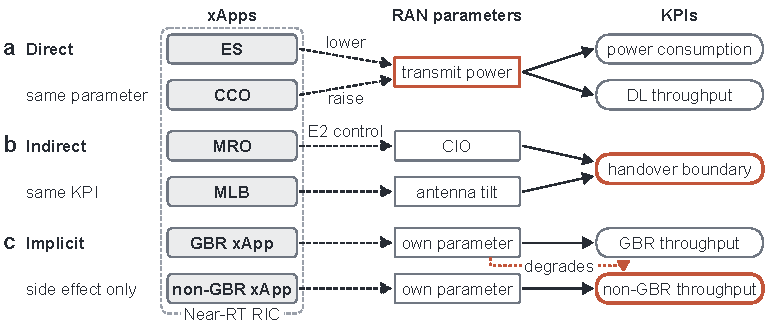
\includegraphics[width=\textwidth]{figures/fig_conflict_types.pdf}
\caption{O-RAN conflict types.}
\label{fig:intro_conflict}
\end{figure}

A growing literature learns such maps from network
data~\cite{QACM2024,PACIFISTA,Sharma_2025,santos2026conflictairan}, but these data are logs written by the controllers
themselves. An xApp issues a request because of the state of its cell, and the same state drives the KPIs, so an
association between requests and KPIs mixes the effect of the request with the controller's reaction to the network.
Relationships learned from such logs are therefore confounded, and a discovery method can report effects where none
exist; in our evaluation, every associational baseline reported edges on placebo logs, in which no parameter has any
effect.

This confounding can be removed within the near-RT RIC itself. Every xApp request already passes through the
conflict-mitigation layer of the RIC, which accepts or rejects it~\cite{ORANRICARCH}, and we call the rule that makes
this choice the referee. If the referee draws each decision at random with a probability that it records, the logs
carry a known experimental design, and redrawing the logged decisions yields a randomisation test of whether a
parameter affects a KPI. Such a test is design-based: its validity rests on the randomisation performed by the
referee rather than on a model of the network, at the cost of rejecting some requests at random while the logs are
collected. We evaluate this approach on three questions: whether a design-based test is valid on such logs, whether
the causal map it learns agrees with an independent ground truth, and whether decisions taken with the map improve on
static rules within the safety limits. The evaluation uses a system-level simulation of an O-RAN surge scenario, in
which energy-saving xApps conflict with a slice-protection xApp, and controlled environments with known causal
structure.

The first two answers are positive. The test declared no effect on placebo logs and never reported an effect with the
wrong sign, and most of the effects it reported were confirmed by a knockout ground truth, on randomised and
confounded logs alike. In the controlled environments, tests that ignored the logging design lost their error control
once the logging followed a dithered setpoint instead of independent draws, whereas tests that used the design kept
it. The third answer is negative: a referee acting on the map reduced protected-slice violations but breached a
radio-link-failure limit, and behind a gate that admits only certified-safe rejections it fell back to the best static
rule, as did the true causal map. In this scenario, the safety guards rather than knowledge of the network limit what
conflict mitigation can achieve.

The paper makes three contributions.
\begin{enumerate}
\item \textbf{The test}. PMRT, a design-based test that learns signed causal effect maps from near-RT RIC request
logs with logged probabilities, with an explicit estimand and the conditions for its asymptotic validity.
\item \textbf{The validity evidence}. Placebo and null-outcome checks on the simulator, and a study on five
controlled environments of whether edge tests keep their error rate when the logging design is known. The evidence
suggests a practical placebo check, a necessary condition only, for learned discovery pipelines on designed logs.
\item \textbf{The decision study}. A test of whether such a map improves safe decisions, with a map-driven referee
and an edge-certification gate. In the evaluated scenario the map gave no such improvement, and this gap between a
valid map and a better safe policy is the paper's central result.
\end{enumerate}
The work builds on our conference paper on causal discovery-driven conflict mitigation, CDD
O-RAN~\cite{dahal2026cddoran}, but replaces its method rather than extending it.
